\begin{itemize}
    \item When moving processing to a high performance cluster there are two main gains:
        \begin{itemize}
            \item Parallelism, which greatly benefits this problem as it is 'embarrassingly parallel'
            \item Serial speed of each compute node (clusters are usually well specified w.r.t. RAM and CPU provisions)
        \end{itemize}
\end{itemize}


\subsection{HEC}

\begin{figure}[h]
    \centering
    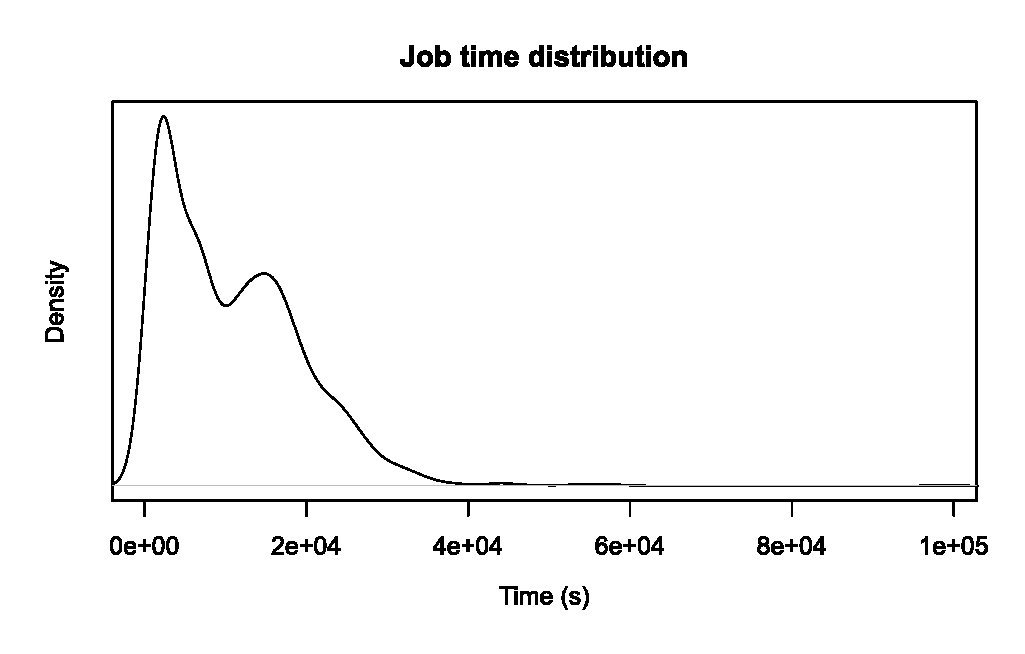
\includegraphics[width=0.5\textwidth]{jobtime.eps}

    \begin{tabular}{ | r | c | c | c | c | c | }
        \hline
        Percentile & 5 & 25 & 50 & 75 & 95 \\ \hline
        Duration & 20m & 53m & 2.5h & 4.5h & 7.3h \\ \hline
    \end{tabular}

    \caption{Distribution of job execution times on the HEC}
    \label{fig:jobtimes}
\end{figure}


% 
% {\small
% \begin{verbatim}
% Total time (s): 24428748    ( / 60 / 60 / 24 = 282 days on the HPC )
% Mean (s): 10955             ( / 60 / 60 = 3.04 hours )
% Min (s): 223                ( / 60 = 3.7 minutes )
% Max (s): 98872              ( / 60 / 60 = 27 hours )
% 
% 
% > quantile(x$time, c(.05, .25, .50, .75, .95))
%        5%       25%       50%       75%       95% 
%  1248.897  3174.155  9321.105 16462.717 26126.913 
%  20 mins   53 mins   2.5 hrs  4.5 hrs   7.25hrs
% \end{verbatim}
% }
% 




Jobs were complete in 3 days, meaning that the system tagged at a rate of 31.5 million words 
%31,555,349 words 
per hour.  Because of the heterogeniety in task length, this rate was not constant, decaying towards the end (the final 300) as the queued tasks ran out.  Had we used larger batches, this effect would have proven more severe as the variance in job length was liable to increase.


Jobs used between 80 and 120MB of memory at maximum point.  Since the HEC  (jobs were not optimised for memory usage and the toolchain is very light on RAM).

"Each task runs all files in 20 directories through the tagger.  The other times are per-task could time info, just to give an idea of the variance.
The minimum is probably flawed because the list of directories was padded to be divisible by 20."

\begin{itemize}
    \item Throughput on HEC
    \item Scalability of HEC setup
\end{itemize}





\subsection{Commodity Hardware}
In many cases, the alternative to deployment on a HEC cluster will be use of one or many commodity desktop machines.  In order to compare the performance of the toolchain, a random sample of 50 jobs was run through the toolchain using the scheduling scripts described above.

The hardware used was a desktop machine with a single Intel i5 processor, 15GB of memory, and two 7200rpm mechanical hard disks in a RAID-0 configuration.  The system was running arch linux\footnote{\url{http://archlinux.org}}, and work continued on other projects during the benchmark.  We believe this constitutes a system equivalent to many found across offices today.

\begin{figure}[h]
    \centering
    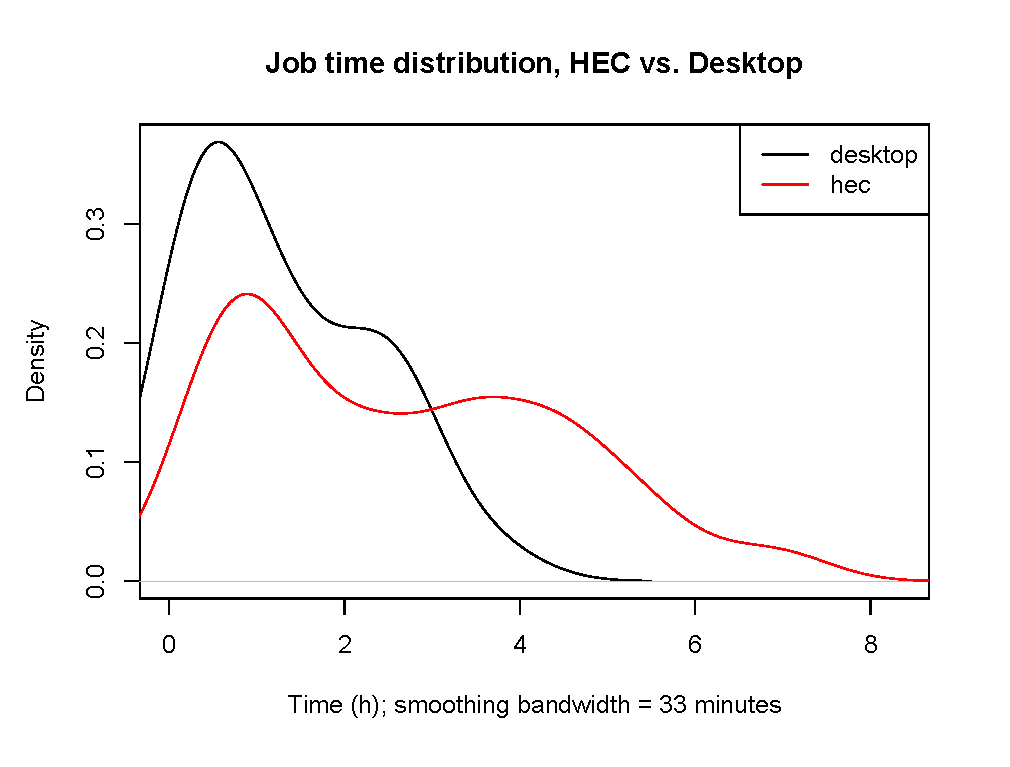
\includegraphics[width=0.5\textwidth]{timecomp.eps}
    % postscript("timecomp.eps", height=5, width=6.5)
    % plot(density(times$tdesk/3600, bw=2000/3600), xlim=c(0, 30000/3600), main="Job time distribution, HEC vs. Desktop", xlab="Time (h); smoothing bandwidth = 33 minutes")
    % lines(density(times$thec/3600, bw=2000/3600), col=2)
    % legend("topright", c("desktop", "hec"), lty=1, col=c(1,2))
    % dev.off();

    % -------------
    % > quantile(times$thec, c(.05, .25, .50, .75, .95))
    %        5%       25%       50%       75%       95% 
    %  1322.534  3404.690  8524.075 14848.393 20306.699 
    % > quantile(times$tdesk, c(.05, .25, .50, .75, .95))
    %         5%        25%        50%        75%        95% 
    %   552.9762  1332.1664  3804.2810  8380.7053 10042.5802 

    \begin{tabular}{ | r | c | c | c | c | c | }
        \hline
        Percentile & 5 & 25 & 50 & 75 & 95 \\ \hline
        HEC        & 22m & 57m & 2.4h & 4.1h & 5.6h \\ \hline
        Desktop    & 9m & 22m & 1h & 2.3h & 2.8h \\ \hline
    \end{tabular}

    \caption{HEC and Desktop job execution times for a sample of 50 jobs}
    \label{fig:timecomp}
\end{figure}


As can be seen in Figure~\ref{fig:timecomp}, the desktop system runs jobs significantly faster.  Fitting a linear model indicates that the desktop is able to run jobs approximately 2.1 times faster than a single HEC core.  

Had we continued to tag the corpus in this manner, it would have taken 98 days on the desktop system.
